\documentclass{beamer}

\usepackage[utf8]{inputenc} % For UTF-8 encoding
\usepackage[T1]{fontenc}    % For better font encoding
\usepackage{graphicx} % For handling images
\usepackage{lipsum}   % For generating dummy text (optional)
\usepackage{tikz}     % For positioning

% Define the x and y shift values as variables (can be adjusted)
\newcommand{\titleXShift}{-0.4cm} % Horizontal shift (left or right)
\newcommand{\titleYShift}{0.2cm} % Vertical shift (up or down)

% Adjust the vertical space between the title and the top edge of the slide for non-title slides
\setlength{\topskip}{20pt} % Space between title and slide content (adjust this)
\setlength{\headheight}{0pt} % Remove any header height
\setlength{\headsep}{10pt}    % Remove any separation between header and content

% Move the frame title using TikZ
\setbeamertemplate{frametitle}{
  \vskip\titleYShift % Shift title vertically
  \hspace*{\titleXShift} % Shift title horizontally
  \insertframetitle % Insert the title itself
}

% Set up the header to place an icon in the top-right corner (optional)
\setbeamertemplate{headline}{
  % Nothing here for the header, we are focusing on the top-right icon
}

% Add the icon to the top-right corner using TikZ (optional)
\addtobeamertemplate{headline}{%
  \begin{tikzpicture}[remember picture,overlay]
    \node[anchor=north east,xshift=-0.5,yshift=-0.5] at (current page.north east) {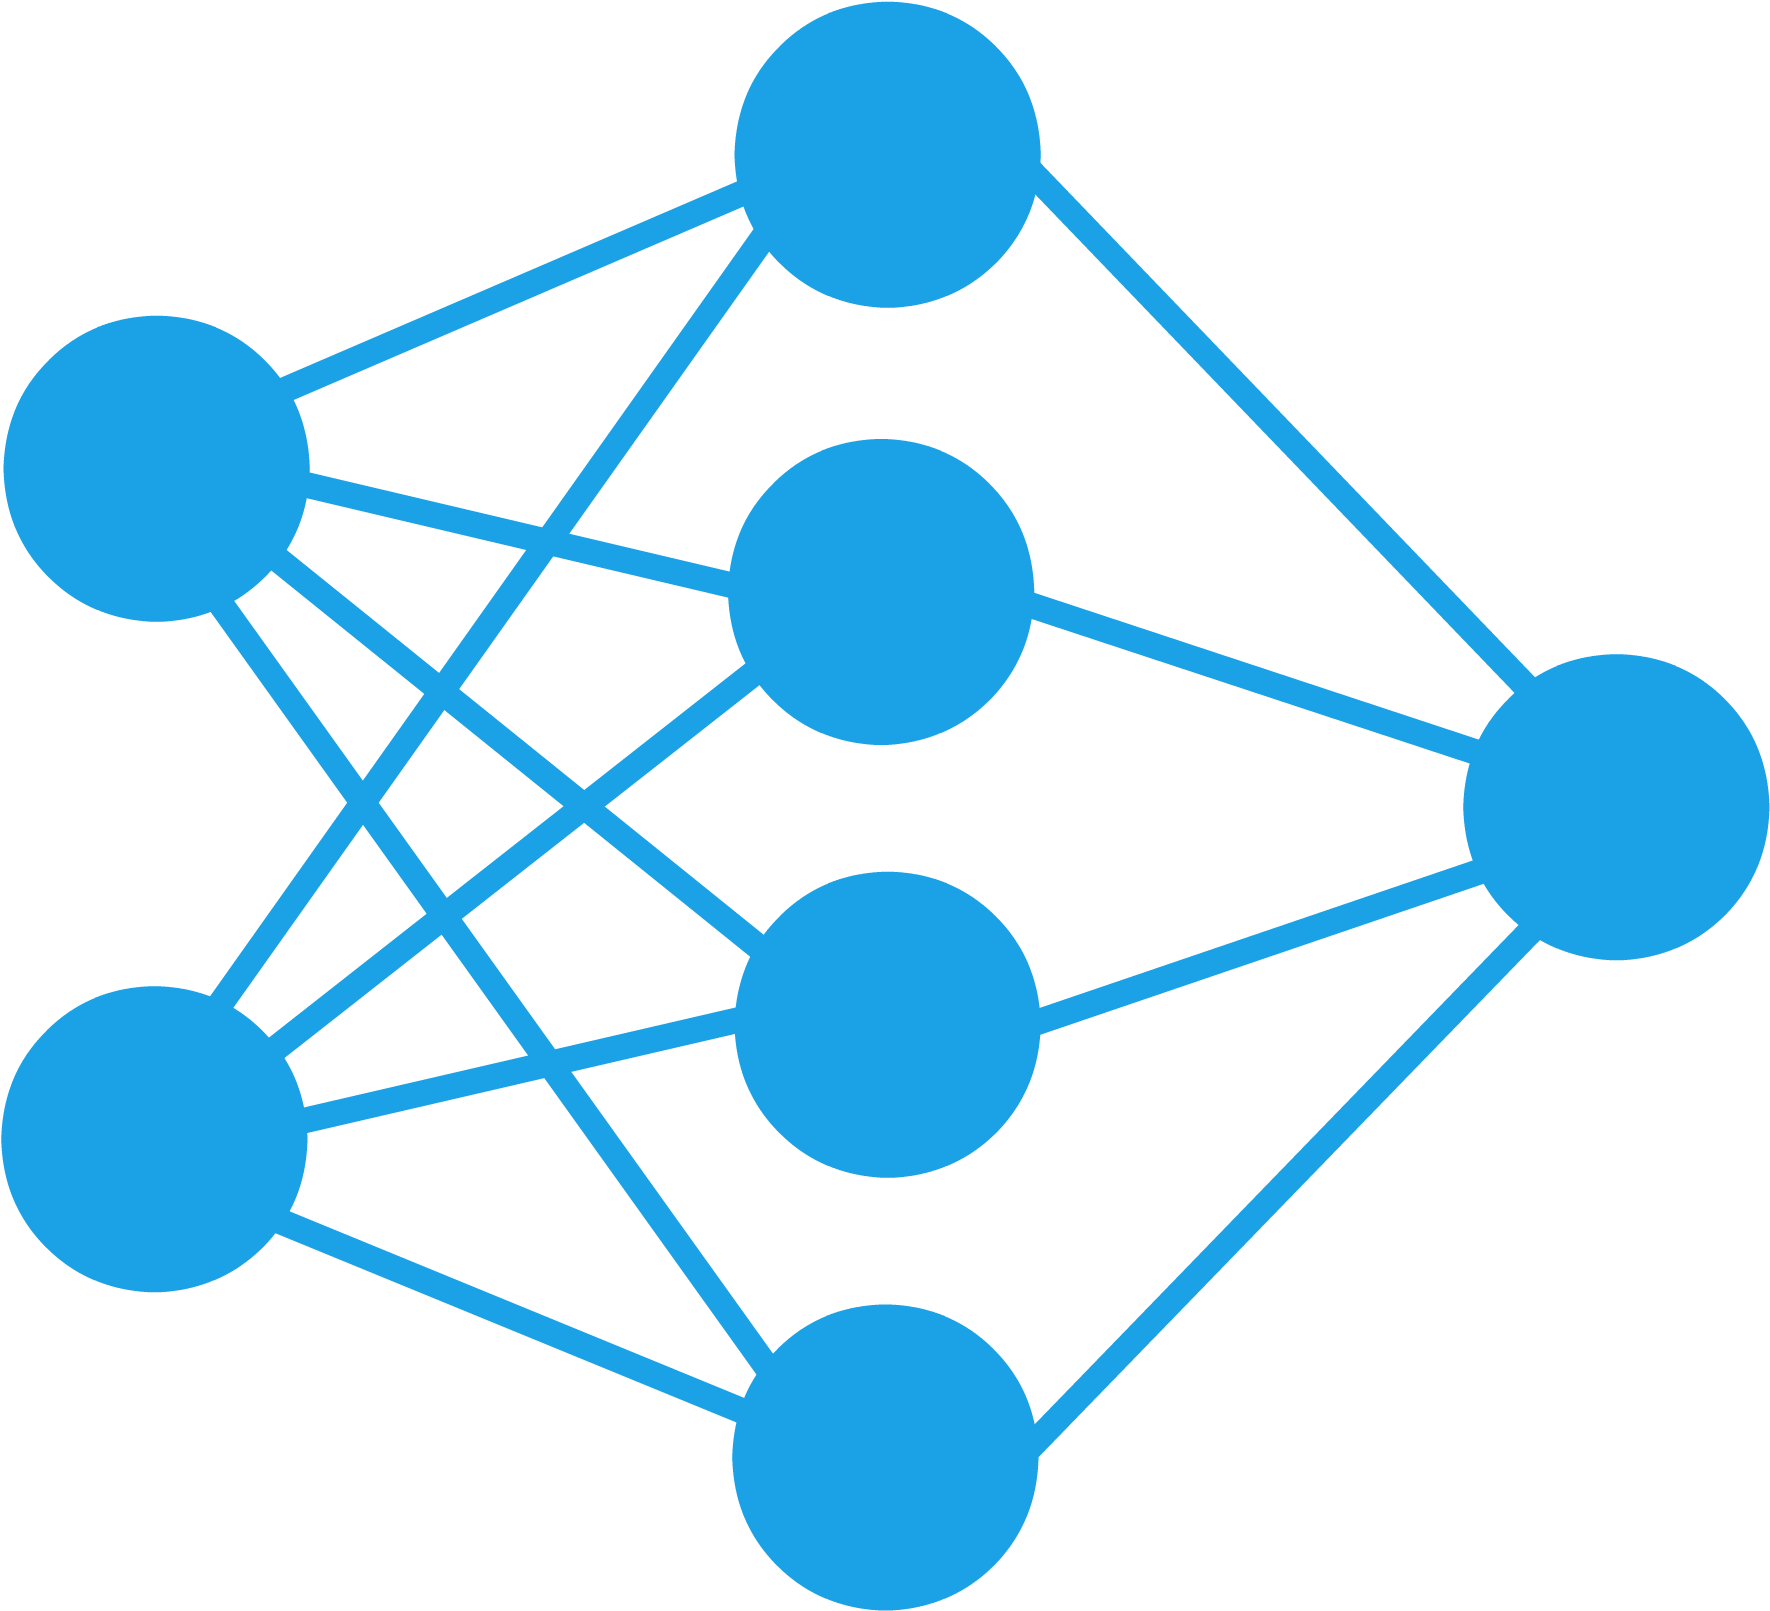
\includegraphics[width=1cm]{pictures/icon.png}};
  \end{tikzpicture}%
}

% Set up the footer with page numbers (optional)
\setbeamertemplate{footline}{
  \begin{beamercolorbox}[wd=\paperwidth,ht=1.0cm,dp=0.5cm,center]{section in head/foot}
    \insertframenumber{} / \inserttotalframenumber
  \end{beamercolorbox}
}

\title{Optimierung der Newsletter Öffnungrate \newline
 Reinforcement Learning}
\author{Simon Schärer}
\date{\today}

\begin{document}

\frame{\titlepage}

\begin{frame}
  \frametitle{Agenda}

  \begin{enumerate}
    \item \hyperlink{sec1}{Ausgangslage}
    \item \hyperlink{sec2}{Idee}
    \item \hyperlink{sec3}{Datengrundlage}
    \item \hyperlink{sec4}{Verteilung Trainingsdatensatz}
    \item \hyperlink{sec5}{Modellübersicht}
    \item \hyperlink{sec6}{Modell-Details}
    \item \hyperlink{sec6}{Leistung}
    \item \hyperlink{sec7}{Klassifizierung der Testdaten}
    \item \hyperlink{sec8}{Learnings / Code}
  \end{enumerate}
\end{frame}


% Ausgangslage
\begin{frame}  
\label{sec1}
	\frametitle{Ausgangslage}
Ich versende monatlich einen Newsletter an ca. 30'000 Kunden mit dem Ziel, dass die Kunden den Newsletter lesen und mit uns interagieren. Als Interaktion zählt nicht nur der Kauf eines Produktes, sondern für mich ist auch schon der Klick auf Text, Blogeintrag etc. wertvoll, damit ich ein Kundenprofil erstellen kann und somit mehr Informationen (Interessen) über den Kunden erfahre.
\\
[0.2cm] % Adds 1cm space between lines
Der Erfolg eines Newsletter kann mittels Öffnungsrate, Klickrate etc. gemessen werden. 
\\
[0.2cm] % Adds 1cm space between lines
Aus meiner vergangen Tätigkeit weiss ich, dass nur schon der Betreff Einfluss auf die Öffnungsrate hat.


%\[Oeffnungsrate = \frac{Anzahl Email Oeffner}{Anzahl Emailversendet}\] 
\end{frame}

% Idee
\begin{frame}  
	\label{sec2}
  	\frametitle{Idee}
 In meinem Beispiel hat jeder Kunden eines der folgenden Intressen:
	\begin{itemize}
	\item Anlegen
	\item Finanzieren
	\item Vorsorge
	\end{itemize}
\vspace{0.2cm}% Adds 1cm space between lines
 Wenn ich den Betreff des Newsletters richtig, also dem Kunden entsprechend richtig treffe, öffnet er den Newsletter und ist für mich ein Erfolg.
 \end{frame}

% Datengrundlage
\begin{frame}  
\label{sec3}
  	\frametitle{Datengrundlage}
Da ich für dieses Experiment keine echten Daten nutzen kann, habe ich alle Daten selber generiert. Dies stellte sich als grössere Herausforderung heraus als ursprünglich gedacht.  

\begin{table}[ht]
\centering
\begin{tabular}{|c|c|c|c|c|}
\hline
Alter &  Finanzieren &  Anlegen &  Vorsorge & Groundtruth \\ \hline
 34 & 0.432 & 0.343 & 0.364 &  Finanzieren  \\ \hline
 56 & 0.128 & 0.531 & 0.358 &  Anlegen  \\ \hline
 45 & 0.985 & 0.365 & 0.663 &  Vorsorge  \\ \hline

\end{tabular}
\caption{Datengrundlage}
\end{table}
\end{frame}


% Verteilung Trainigsdatensatz
\begin{frame}
\label{sec4}
  	\frametitle{Verteilung Trainingsdatensatz}
  \centering
  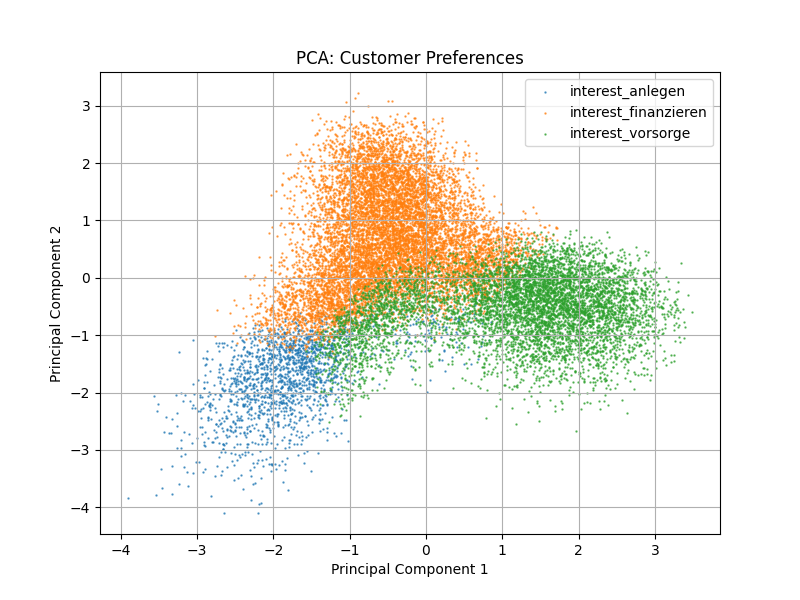
\includegraphics[width=0.65\textwidth]{figures/pca_groundtruth_s05.png}
  
  \begin{block}{Klarer Unterschied}
 Ich musste sicherstellen, dass der RL Algorithmus auch etwas lernen kann, sonst wusste ich nicht, ob die Daten oder mein Algorithmus schlecht ist. Deshalb habe ich meine Daten so erstellt, dass sie klar unterschiedlich sind.
  \end{block}
\end{frame}


%
%% Lösung
%\begin{frame}
%\label{sec5}
%  	\frametitle{Lösung}
%Bis ich eine halb brauchbare Lösung gefunden habe musste ich einiges Ausprobieren. Ich versuchte es zuerst mit einem Q-Table, habe ich mich aber nachher dazu entschlossen es mit einem einfachen Q-Network zu probieren.
%\end{frame}


% Modellübersicht
\begin{frame}
    \label{sec5}
    \frametitle{Modellübersicht}
%    \textbf{Ziel:} Optimierung der Kundenzielgruppenansprache in der Finanzbranche durch Erlernen von Präferenzen und Vorhersage optimaler Kundenaktionen.

    \begin{itemize}
        \item \textbf{Ansatz:} Modell mit einem DQN-basierten Agenten (Deep Q-Network).
        \item \textbf{Umgebung:} Simulation von Betreff mit drei Finanzthemen:
        \begin{itemize}
            \item \textbf{Anlegen}, \textbf{Finanzieren}, \textbf{Vorsorge}.
        \end{itemize}
        \item \textbf{Zustandsrepräsentation:}
        \begin{itemize}
            \item Merkmale: Alter, finanzielle Interessen (Anlegen, Finanzieren, Vorsorge)           
            \item  Standardisiert (standardscaler) für bessere Repräsentation.
        \end{itemize}
        \item \textbf{Aktionen:} Auswahl eines der drei Finanzthemen basierend auf vorhergesagten Präferenzen.
    \end{itemize}
\end{frame}

% Modell-Details
\begin{frame}
    \label{sec6}
    \frametitle{Modell-Details}

    \textbf{Agent:}
    \begin{itemize}
        \item \textbf{Architektur:} Deep Q-Network (Policy- und Zielnetzwerke).
        \item \textbf{Hyperparameter:}
        \begin{itemize}
            \item Lernrate: 0.001
            \item Diskontfaktor ($\gamma$): 0.95
            \item Epsilon-Verfall: 0.9
            \item Ziel-Netzwerk-Update-Frequenz: alle 10 Schritte
        \end{itemize}
        \item \textbf{Reward Funktion:}
        \begin{itemize}
            \item Richtiges Thema: $+3$
            \item Falsches Thema: $-1$
        \end{itemize}
    \end{itemize}

%    \textbf{Datensatz:}
%    \begin{itemize}
%        \item \textbf{Generierter Datensatz:}
%        \begin{itemize}
%            \item 30.000 Proben, 60\% Training, 40\% Test.
%            \item Attribute: Alter, Verbindlichkeiten, Geschlecht und finanzielle Interessen.
%            \item Ground Truth: Bevorzugtes Thema, basierend auf Zinsbewertungen.
%        \end{itemize}
%    \end{itemize}

    
\end{frame}


\begin{frame}
\label{sec7}
\frametitle{Leistung}

\centering

% Two figures side by side
\begin{columns}
    \column{0.5\textwidth}
    \begin{figure}
        \centering
        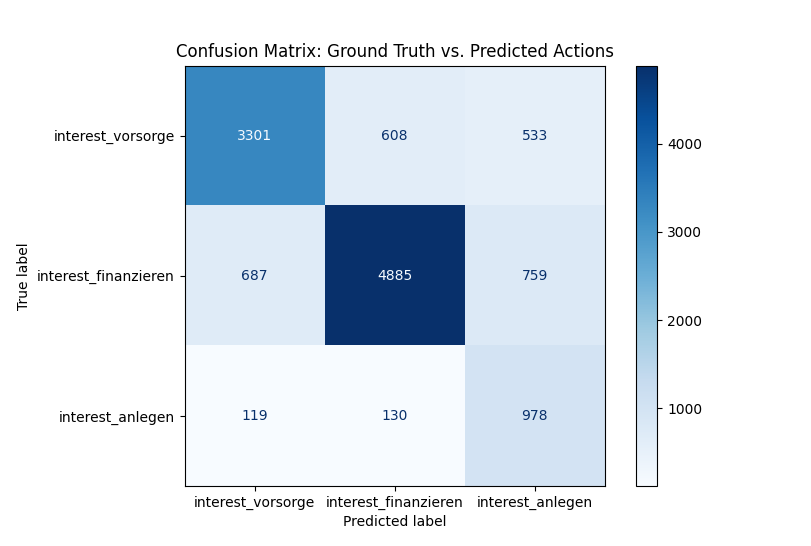
\includegraphics[width=1\textwidth]{figures/cm.png}
        \caption{Absolute Werte}
    \end{figure}
    
    \column{0.5\textwidth}
    \begin{figure}
        \centering
        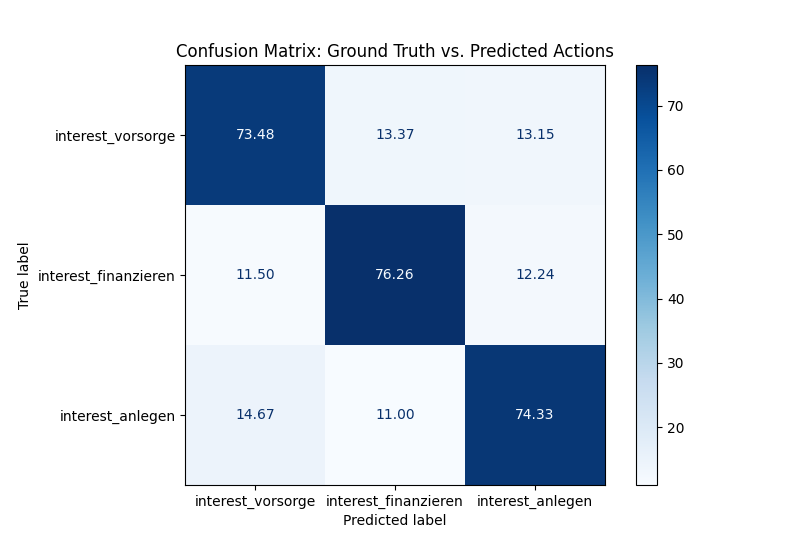
\includegraphics[width=1.\textwidth]{figures/cm_pct.png}
        \caption{Relative Werte}
    \end{figure}
\end{columns}

\vspace{0.1cm} % Adjust space between figures and text

% Text box below the figures
\begin{block}{}
\textbf{Leistung}
    \begin{itemize}
        \item \textbf{Metriken:} Konfusionsmatrix, Accuracy (ca. 75\% mit optimierten Parametern).
        \item \textbf{Bewertung:} Vergleich der vorhergesagten Aktionen mit Ground Truth.
    \end{itemize}
\end{block}

\end{frame}




% Klassifizierung Testdaten
\begin{frame}
\label{sec8}
 \frametitle{Klassifizierung der Testdaten}
 \centering
  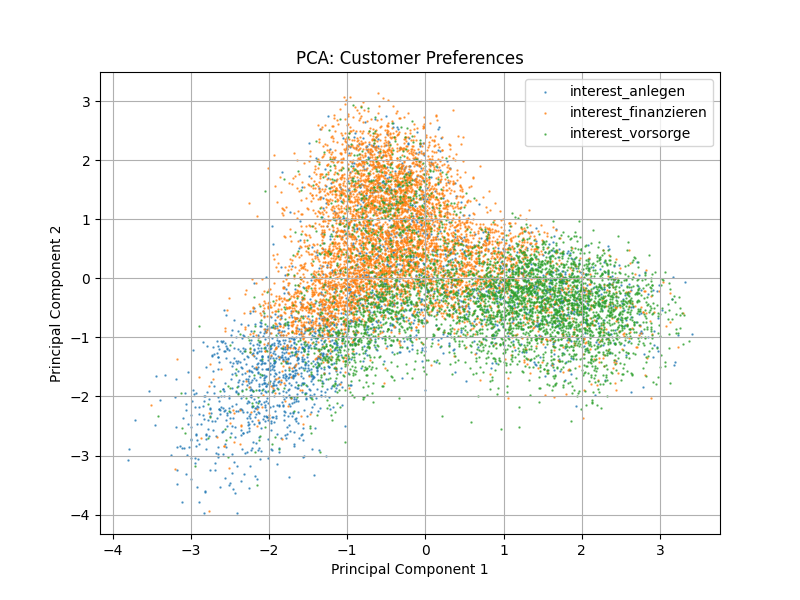
\includegraphics[width=0.65\textwidth]{figures/pca_test_data_action_small.png}
  
    \begin{block}{Testdaten}
  Die Cluster und die Interessen Zugehörigkeit sind ersichtlich und stimmen grösstenteils.
  \end{block}
   
  
\end{frame}


% Code
\begin{frame}  
	\label{sec9}
  	\frametitle{Learnings / Code}
  	\textbf{Learnings:}
  	\begin{itemize}
	\item Ziel muss klar und am Anfang einfach sein, musste die Zielkomplexität mehrfach nach unten anpassen.
	\item Daten waren aufwändig zu generieren.
	\item Architektur, Hyperparameter, Reward-Funktion... es gibt viele Stolpersteine.
	\item ohne ChatGPT wäre ich immer noch am debuggen...
	\end{itemize}
	
	\textbf{Code:}
	\begin{itemize}

	\item \url{https://github.com/ssch-fpv/lr_newsletter}
	\end{itemize}

 \end{frame}

\end{document}
